\documentclass[12pt,a4paper]{article}
\usepackage{graphicx}
\usepackage{hyperref}
\usepackage{wrapfig}
\setlength{\headheight}{12pt} 
\setlength{\textheight}{25cm}
\setlength{\textwidth}{17cm}
\setlength{\footskip}{10mm}
\setlength{\oddsidemargin}{0mm}
\setlength{\evensidemargin}{0mm}
\setlength{\topmargin}{0mm}
\setlength{\headsep}{10mm}
\usepackage{geometry}
\usepackage{fancyhdr}
\usepackage[T1]{fontenc}
\usepackage[polish]{babel}
\usepackage[utf8]{inputenc}
\usepackage{lmodern}
\selectlanguage{polish}
\newgeometry{rmargin=2cm,lmargin=2cm,bmargin=2cm}
\pagestyle{fancy} %naglowek
\rhead{Albert Szadziński}
\chead{}
\lhead{\thepage\hspace{0.5cm} FlaskApp}
\lfoot{ }
\usepackage{listings}
\cfoot{ }
\rfoot{}
\begin{document}

\thispagestyle{empty}
\begin{center}
{\huge \textbf{Dokumentacja}\\[2.7in]}

\textbf{{\LARGE Aplikacja HelpDesk\\ FlaskApp}}\\

{\large v1.5}\\[4.7in]
\end{center}
\begin{flushright}
\begin{large}
16 wrzesień 2017\\
Albert Szadziński

\end{large}
\end{flushright}


\newpage
\tableofcontents
\newpage

\section{Instalacja}
\subsection{Wersje oprogramowania}
\begin{itemize}
\item \textbf{System operacyjny} \\
\textit{Ubuntu 16.04 xenial - wersja serwerowa\\
Linux ubuntu 4.4.0-87-generic}
\item \textbf{apache2}\\
\textit{Server version: Apache/2.4.18 (Ubuntu)\\
Server built:   2017-07-27T14:34:01}
\item \textbf{MySQL}\\
\textit{mysql 14.14 Distrib 5.7.19}
\item \textbf{pip}\\
\textit{pip 8.1.1 from /usr/lib/python2.7/dist-packages (python 2.7)}
\item \textbf{Flask} \\
\textit{Flask 0.12.2\\
Python 2.7.12 (default, Nov 19 2016, 06:48:10) \\}
\end{itemize}


\subsection{Konfiguracja środowiska do wirtualizacji}
\quad

Po instalacji aktualnej wersji \textbf{VirtualBoxa} należy przejść do \textit{File>Import} w przypadku posiadania obrazu systemu \textbf{.ova } lub do \textit{File>New } aby rozpocząć instalację nowego systemu z obrazu \textbf{.iso}. W obu przypadkach należy zatwierdzić domyślne konfiguracje.\\

Przed uruchomieniem maszyny wirtualnej należy upewnić się, czy włączone jest mostkowanie karty sieciowej na aktualnie używanym interfejsie sieciowym. 
\begin{figure}[h!]
\centering
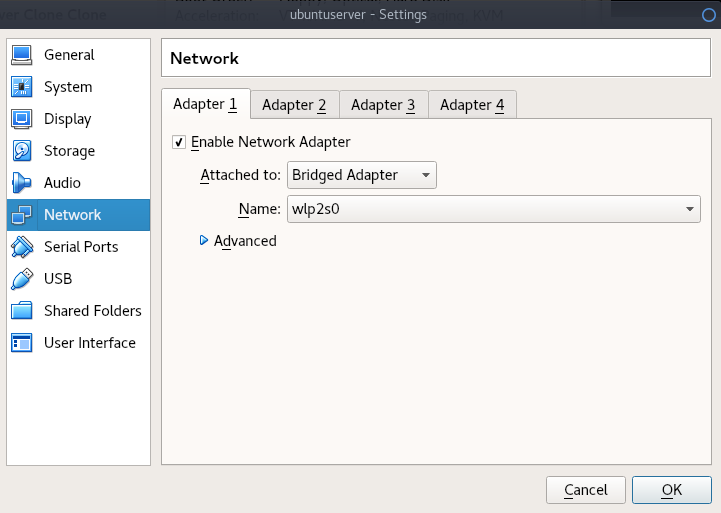
\includegraphics[scale=0.4]{d}
\end{figure}
\newpage

\subsection{Instalacja pakietów}
\quad
W przypadku importowania maszyny z pliku .ova wszystkie niezbędne pakiety są zainstalowane, a poniższe instrukcje należy zastosować w momencie wystąpienia problemów w działaniu aplikacji od punktu \textbf{(1.4.3)} po wcześniejszym wykonaniu:
\begin{lstlisting}
$: rm -rf /var/www/FlaskApp/FlaskApp/venv  #jako root
\end{lstlisting}
\quad

Po uzyskaniu dostępu do VM (maszyna wirtualna) poprzez VBox lub SSH należy przejść na użytkownika \textit{root}:\\
\begin{lstlisting}
$: sudo su #lub
$: su
\end{lstlisting}

Domyślne hasła:
\begin{itemize}
\item server:0e48e4Jmmr
\item root:4oo1Jmmr
\end{itemize}

\textbf{Aktualizacja listy oraz pakietów:}
\begin{lstlisting}
$: apt-get update
$: apt-get upgrade
\end{lstlisting}

\textbf{Instalacja niezbędnych pakietów:}
\begin{lstlisting}
$: apt-get install apache2 mysql-client mysql-server libapache2-mod-wsgi
 libmysqlclient-dev python-dev python-pip phpmyadmin 
 texlive texlive-lang-polish texlive-fonts-extra python-mysqldb
\end{lstlisting}

\subsection{Konfiguracja serwera}

\subsubsection{Tworzenie katalogu na aplikacje}
\begin{lstlisting}
$: mkdir /var/www/FlaskApp
\end{lstlisting}
\subsubsection{Pobieranie kodu źródłowego aplikacji wraz z szablonami}
\begin{lstlisting}
$: cd /var/www/FlaskApp
$: git clone https://github.com/aszadzinski/help-desk-panel
$: mv help-desk-panel/ FlaskApp/
\end{lstlisting}
\subsubsection{Tworzenie wirtualnego środowiska dla webaplikacji}
\begin{lstlisting}
$: pip install virtualenv
$: cd /var/www/FlaskApp/FlaskApp
$: virtualenv venv
\end{lstlisting}
\newpage
\subsubsection{Instalacja lokalnych modułów dla Pythona i test aplikacji}
\begin{lstlisting}
$: source venv/bin/activate
(venv)$: pip install flask
(venv)$: pip install mysql-python
(venv)$: pip install mysql 
(venv)$: python __init__.py
\end{lstlisting}
Po wykonaniu ostatniego polecenia w terminalu powinny pojawić się informacje o rozpoczęciu nasłuchiwania na localhoscie:
\begin{lstlisting}
(venv) root@ubuntu:/var/www/FlaskApp/FlaskApp# python __init__.py 
 * Running on http://127.0.0.1:5000/ (Press CTRL+C to quit)
 * Restarting with stat
 * Debugger is active!
 * Debugger PIN: 717-628-278
\end{lstlisting}
po otrzymaniu takiej odpowiedzi należy je anulować CTRL+C oraz wyjść z virtualenv:
\begin{lstlisting}
(venv)$: deactivate
\end{lstlisting}
W przypadku otrzymania błędu należy doinstalować brakujące moduły widoczne w komunikacjie błędu jako np: 
\begin{lstlisting}
Line 12: import MySQLdb 
module not found
\end{lstlisting}
poprzez wpisanie w środowisku wirtualnym:
\begin{lstlisting}
$: pip install <modul>
\end{lstlisting} 
lub przez manager pakietów:
\begin{lstlisting}
$: apt-get install python-<modul>
\end{lstlisting}

\subsubsection{Konfiguracja apache2}

Po uzyskaniu poprawnego działania na localhoscie należy dodać aplikacje FlaskApp do stron apache'a oraz uruchomić mod \textit{wsgi}.\\

Aktywacia wsgi:
\begin{lstlisting}
$: a2enmod wsgi
$: service apache2 restart
$: touch /var/www/FlaskApp/flaskapp.wsgi
\end{lstlisting}
do pliku flaskapp.wsgi wkleić należy:
\begin{lstlisting}
import sys
import logging
logging.basicConfig(stream=sys.stderr)
sys.path.insert(0,"/var/www/FlaskApp/")
from FlaskApp import app as application
application.secret_key = 'foobarspameggs'
\end{lstlisting}
\newpage

Następnie po stowrzeniu pliku:
\begin{lstlisting}
$: touch /etc/apache2/sites-available/FlaskApp.conf
\end{lstlisting}

z zawartością:
\begin{lstlisting}
<VirtualHost *:80>
                ServerName <aktualny adres IP VM>
                ServerAdmin jakis@mail.com
                WSGIScriptAlias / /var/www/FlaskApp/flaskapp.wsgi
                <Directory /var/www/FlaskApp/FlaskApp/>
                        Order allow,deny
                        Allow from all
                </Directory>
                Alias /static /var/www/FlaskApp/FlaskApp/static
                <Directory /var/www/FlaskApp/FlaskApp/static/>
                        Order allow,deny
                        Allow from all
                </Directory>
                ErrorLog ${APACHE_LOG_DIR}/error.log
                LogLevel warn
                CustomLog ${APACHE_LOG_DIR}/access.log combined
</VirtualHost>
\end{lstlisting}     
 
należy dodać aplikację do aktywnych: 
\begin{lstlisting}
$: a2ensite FlaskApp
$: service apache2 reload
\end{lstlisting}
\newpage
\section{Konfiguracja aplikacji}
\subsection{Pliki konfiguracyjne aplikacji}
\subsubsection{Zarządzanie działami i typami zleceń}
\quad
W katalogu aplikacji \textit{/var/www/FlaskApp/FlaskApp}  w folderze \textit{config\_files} zdajdują się pliki konfiguracyjne odpowiedzialne za:
\begin{itemize}
\item Działy (\textit{branches.data}):\\
Każda linia tego pliku interpretowana jest przez program jako nowy dział
\item Typy zleceń (\textit{typy\_zleceń.config}\\
jak wyżej
\item Incydenty (incydenty.config)\\
Linie rozpoczynające się od \# oraz od znaku nowej lini są ignorowane.\\
Linie rozpoczynające się od spacji traktowane są jako opcja wyboru do najbliższej lini nad ną nie rozpoczynającej się od spacji
\end{itemize}
\subsubsection{Podpinanie bazy danych pod aplikacje}
Pośrednikiem między aplikacją FlaskApp a bazą MySQL jest skrytp \textit{database\_connect.py} do którego odwołuje się skrypt \textit{db\_func.py} z zapytaniami sql. Aby zmienić aktualną bazę należy zmodyfikować parametry metody MySQLdb.connect w pliku database\_connect.py:
\begin{lstlisting}
conn = MySQLdb.connect(host="localhost", user = "root",
                     passwd = "3y0q5rZkn", db = "helpdesk")
\end{lstlisting}

\subsection{Zarządzanie bazą danych}
Domyślne hasło bazy MySQL na pliku .ova:\\
root: 3y0q5rZkn

\subsubsection{Zarządzanie użytkownikami}
\quad
Aplikacjia umożliwia dostęp do bazy użytkownikow z poziomu panelu admina po zalogowaniu lub przez phpmyadmin (tabela users). \\

Domyślne hasło admina:\\
admin: changeme

Pole "Uprawnienia" jest istotne dla programu tylko w momencie gdy przyjmuje wartość " admin", inne wartości są ignorowane i przydzielają użytkownika do grupy bez uprawnień.\\

\subsubsection{Wiadomości i aktualności(tabele news i notifications)}
\quad
W przypadku posiadania przez użytkownika uprawnień admina może od publikować wiadomości z zakładki aktualności widoczne dla każdego użytkownika oraz zarządzać przychodzacymi zleceniami.
Każdy admin w zakładce Lista zleceń ma dostęp do edycji, zamrażania(ukrycie zlecenia, widoczne tylko w zakładce 'zamrożone') oraz delegowania do innych użytkowników z uprawnieniami admina (widoczne w zakładce 'nowe(do mnie)').\\

W momencie wpisania dowolnej treści w pole 'data zakonczenia' zlecenie przenoszone jest do zakładki 'zakończone'
  \\
\begin{center}
TODO!!!
\end{center}

\section{Aktualizacja}
\subsection{Kopia zapasowa}
\quad
Kopie zapasowe można wykonać poprzez:
\begin{enumerate}
\item Wyeksportowanie do pliku .ova\\
Należy wyłączyć serwer a następnie przejść do zakładki file>export w oknie Virtualboxa
\item Klonowanie maszyny wirtualnej\\
Po wyłączeniu maszyny klinając na nią PPM wybrać Clone
\end{enumerate}

\subsection{Aktualizacja}
\subsubsection{Aktualizacja ze zdalnego repozytorium}
\quad
Maszynie Matce należy należy dać dostęp do globalnej sieci a następnie zresetować VM (konieczne wyłączenie statycznego adresu ip w /etc/network/interfaces).\\   

W momencie uzyskania  dostępu do sieci, w katalogu /var/www/FlaskApp/Flask należy wykonać:
\begin{lstlisting}
$: cd /var/www/FlaskApp/FlaskApp/
$: git checkout master
$: git pull origin master
$: service apache2 reload
\end{lstlisting}
W przypadku błędu, przed poleceniuem pull należy wykonać \textit{git stash}, lub wymusić reset:
\begin{lstlisting}
$: git reset --hard origin/master
\end{lstlisting}
Wpisując polecenie \textit{git log} wyświetli się lista wszystkich zmian kodu, aby przywrócić poprzedną wersje należy wykonać:
\begin{lstlisting}
$: git checkout <id commita>
\end{lstlisting}
\quad

Powyższe instrukcje dotyczą głównej gałęzi programu \textit{master}, aby przełączyć się na gałąź testową \textit{testing} należy wykonać:
\begin{lstlisting}
$: git branch testing
$: git checkout testing
$: git pull origin testing
$: service apache2 reload
\end{lstlisting}
Lub w przypadku wykonania \textit{git reset --hard origin}
\begin{lstlisting}
$: git branch #wyswietla dostepne galezie
$: git checkout testing #wersja testowa
$: service apache2 reload
$: git checkout master #powrot do galezi glownej
\end{lstlisting}
Po aktualizacji i ponownym podłączeniu do sieci lokalnej należy zresetować VM i przywrócić poprzednią konfiguracje w /etc/network/interfaces
\subsubsection{Tworzenie lokalnego repozytorium do aktualizacji}
\begin{center}
TODO!!!
\end{center}
\subsubsection{Pobieranie obrazu VM}
Obraz serwera do importu można pobrać z:\\
 \url{https://drive.google.com/open?id=0B8ey2GDfV593LUFtU1dpUXh2NDQ}

\newpage
\section{Kontakt}
\begin{itemize}
\item Albert Szadziński\\
\begin{itemize}
\item github:\\ \textbf{\url{https://github.com/aszadzinski}}
\item email:\\ \textbf{\url{albert.szadzinski@gmail.com}}
\item klucz PGP\\
\textbf{2F0A E6D3 BEBC BF4E 944E\\
7017 8AC6 85EE 7791 AC83\\}
\url{https://www.facebook.com/glikoliza/publickey/download/}
\end{itemize}
\end{itemize}
\newpage
\section{Ostatnie zmiany}
\begin{itemize}
\item v1.7\\ 
20.09.17
\begin{itemize}
\item aktualizacja dokumentacji (aktualizacja)
\item tymaczasowe ukrycie opcji załącznik
\item naprawa opcji drukowanie
\end{itemize}
\end{itemize}
\end{document}
